%
% kubisch.tex
%
% (c) 2020 Prof Dr Andreas Müller, Hochschule Rapperswil
%
\begin{figure}
\centering
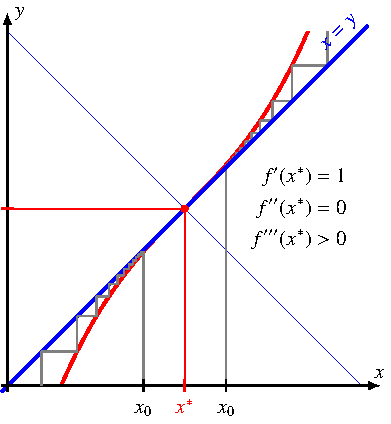
\includegraphics{chapters/10-arithmetik/figures/m1kp.pdf}
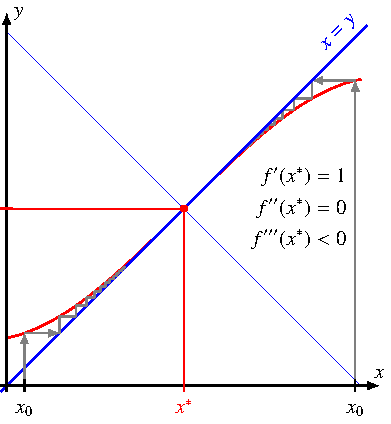
\includegraphics{chapters/10-arithmetik/figures/m1kn.pdf}
\caption{Die Fixpunktiteration $x_{n+1}=f(x_n)$ mit Fixpunkt $x^*$
mit $f'(x^*)=1$ und $f''(x^*)=0$ divergiert für $f'''(x^*)>0$
und konvergiert sehr langsam für $f'''(x^*)<0$.
\label{buch:figure:fixpunkt:abl1kub}}
\end{figure}
%
\begin{figure}
\centering
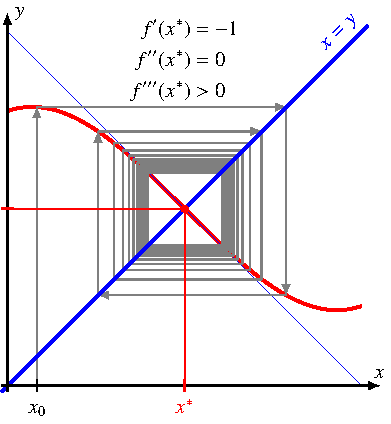
\includegraphics{chapters/10-arithmetik/figures/mnkp.pdf}
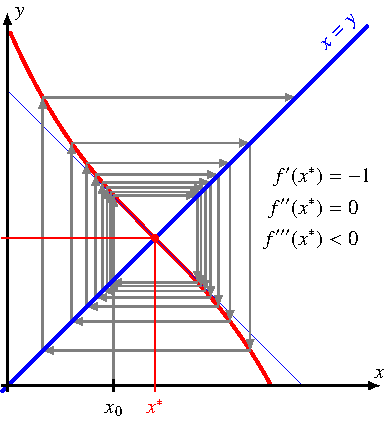
\includegraphics{chapters/10-arithmetik/figures/mnkn.pdf}
\caption{Die Fixpunktiteration $x_{n+1}=f(x_n)$ mit Fixpunkt $x^*$
mit $f'(x^*)=-1$ und $f''(x^*)=0$ konvergiert sehr langsam für $f'''(x^*)>0$
und divergiert für $f'''(x^*)<0$.
\label{buch:figure:fixpunkt:ablm1kub}}
\end{figure}
